\documentclass[a4paper,12pt, oneside]{book}

%\usepackage{fullpage}
\usepackage[italian]{babel}
\usepackage[utf8]{inputenc}
\usepackage{amssymb}
\usepackage{amsthm}
\usepackage{graphics}
\usepackage{amsfonts}
\usepackage{listings}
\usepackage{amsmath}
\usepackage{amstext}
\usepackage{engrec}
\usepackage{rotating}
\usepackage[safe,extra]{tipa}
\usepackage{showkeys}
\usepackage{multirow}
\usepackage{hyperref}
\usepackage{microtype}
\usepackage{enumerate}
\usepackage{braket}
\usepackage{marginnote}
\usepackage{pgfplots}
\usepackage{cancel}
\usepackage{polynom}
\usepackage{booktabs}
\usepackage{enumitem}
\usepackage{framed}
\usepackage{pdfpages}
\usepackage{pgfplots}
\usepackage[cache=false]{minted}
\usepackage{fancyhdr}
\pagestyle{fancy}
\fancyhead[LE,RO]{\slshape \rightmark}
\fancyhead[LO,RE]{\slshape \leftmark}
\fancyfoot[C]{\thepage}



\title{Linguaggi di Programmazione}
\author{UniShare\\\\Davide Cozzi\\\href{https://t.me/dlcgold}{@dlcgold}\\\\Gabriele De Rosa\\\href{https://t.me/derogab}{@derogab} \\\\Federica Di Lauro\\\href{https://t.me/f_dila}{@f\textunderscore dila}}
\date{}

\pgfplotsset{compat=1.13}
\begin{document}
\maketitle

\definecolor{shadecolor}{gray}{0.80}

\newtheorem{teorema}{Teorema}
\newtheorem{definizione}{Definizione}
\newtheorem{esempio}{Esempio}
\newtheorem{corollario}{Corollario}
\newtheorem{lemma}{Lemma}
\newtheorem{osservazione}{Osservazione}
\newtheorem{nota}{Nota}
\newtheorem{esercizio}{Esercizio}
\tableofcontents
\renewcommand{\chaptermark}[1]{%
\markboth{\chaptername
\ \thechapter.\ #1}{}}
\renewcommand{\sectionmark}[1]{\markright{\thesection.\ #1}}
\chapter{Introduzione}
\textbf{Questi appunti sono presi a lezione. Per quanto sia stata fatta una revisione è altamente probabile (praticamente certo) che possano contenere errori, sia di stampa che di vero e proprio contenuto. Per eventuali proposte di correzione effettuare una pull request. Link: } \url{https://github.com/dlcgold/Appunti}.\\
\textbf{Grazie mille e buono studio!}
\chapter{I linguaggi}
Si possono classificare in 3 gruppi i linguaggi di programmazione:
\begin{enumerate}
\item \textbf{Linguaggi imperativi}, come \textit{C, Assembler, Python etc...}. Le caratteristiche dei linguaggi imperativi sono legate all'architettura di Von Neumann, composta da una componente passiva (la memoria) e una attiva (il processore). Il processore esegue calcoli e assegna valori a varie celle di memoria. Si ha quindi il concetto di \textit{astrazione}. Una variabile non è altro che un'astrazione di una cella di memoria fisica. Ogni linguaggio ha diversi livelli di astrazione dell'archiettura di Von Neumann (che ricordiamo usare il "ciclo" formato da \textit{Fetch instruction, Execute e Store result}), con i cosiddetti linguaggi di \textit{alto} e \textit{basso} livello. Possono essere sia linguaggi compilati (come \textit{C}) che interpretati (come \textit{Python}).\\
I linguaggi imperativi usano quindi il \textit{Paradigma Imperativo}, detto anche \textit{Procedurale}. In questo paradigma si adotta uno \textit{stile prescrittivo}, si prescrivono infatti operazioni che il processore deve eseguire e le istruzioni vengono eseguite in ordine, al più di strutture di controllo, e per questo è il miglior paradigma per rappresentare gli algoritmi. Questi linguaggi sono tra i più vecchi e tutt'ora tra i più usati soprattutto per la manipolazione numerica. Si ha la seguente formula che ben descrive il paradigma imperativo:
\begin{center}
\textit{Programma = Algoritmi + Strutture Dati}
\end{center}
In un linguaggio imperativo si ha sia una parte dedicata alla dichiarazione di variabili che una parte dedicata agli algoritmi risolutivi del problema. Inoltre le istruzioni possono essere così divise:
\begin{itemize}
\item istruzioni di I/O
\item istruzioni di assegnamento
\item istruzioni di controllo
\end{itemize}
La ricerca di gestire applicazioni ancora a più alto livello con codice più conciso e semplice, che affrontano i problemi in maniera più logica (o comunque in maniera differente) ha portato alla nascita di altri paradigmi. Linguaggi logici e funzionali sono accomunati dall'essere di altissimo livello, dall'essere generati per manipolazione simbolica e non numerica, dal non distinguere perfettamente programma e strutture dati, dall'essere basati su concetti matematici e sull'adottare uno \textit{stile dichiarativo}
\item \textbf{Linguaggi a oggetti}, come \textit{C++} utilizzano il paradigma ad oggetti con l'uso di classi etc. Non vengono affrontati nel corso.
\item \textbf{Linguaggi Logici}, come il \textit{Prolog}. Si basano sul concetto della deduzione logica e hanno come base la logica formale e come obbiettivo la formalizzazione del ragionamento. Programmare con un linguaggio logico significa descrivere un problema con frasi del linguaggio (ovvero con formule logiche) e interrogare il sistema che effettua deduzioni sulla base della conoscenza rappresentata. Il paradigma logico si può rappresentare con la seguente formula:
\begin{center}
\textit{Programma = Conoscenza + Controllo}
\end{center}
Si ha uno \textit{stile dichiarativo} in quanto la conoscenza del problema è espressa indipendentemente dal suo utilizzo (si usa il \textbf{cosa} e non il \textbf{come}). Si ha quindi un'alta modularità e flessibilità ma si ha la problematica della rappresentazione della conoscenza, infatti definire un linguaggio logico significa definire come il programmatore può esprimere la conoscenza e quale tipo di controllo si può utilizzare nel processo di deduzione.\\
Analizziamo le basi del Prolog:
\begin{itemize}
\item dopo ogni asserzione si mette un \textit{.} mentre le \textbf{,} sono degli \textit{and} logici
\item le costanti si indicano in minuscolo e le variabili in maiuscolo
\item \textbf{Asserzioni Incondizionate (fatti)} così indicate:
\begin{minted}{prolog}
A.
\end{minted}
\item \textbf{Asserzioni Condizionate (regole)}, che ricordiamo non essere regole di inferenza, così indicate:
\begin{minted}{prolog}
A :- B, C, D, ..., Z.
\end{minted}
dove A è il \textit{conseguente}, ovvero la conclusione, mentre le altre sono gli antecedenti, ovvero le premesse. Il simbolo ":-" è un implica che per ragioni di interprete si legge al contrario rispetto al solito: seguendo l'esempio si ha che \textit{B, C, D, ..., Z implicano A} ovvero $B, C, D, ..., Z \to A$
\end{itemize}
\item \textbf{Interrogazione}, che rappresenta l'input utente, è così espressa:
\begin{minted}{prolog}
:- K, L, M, ..., P.
\end{minted}
e indica che si chiede cosa implicano quei dati antecedenti.

Vediamo un esempio più completo (anche se non del tutto):\\
\textit{due individui sono colleghi se lavorano per la stessa 
ditta:}
\begin{minted}{prolog}
collega(X, Y) :- 
     lavora(X, Z), 
     lavora(Y, Z), 
     diverso(X, Y).

lavora(ciro, ibm).
lavora(ugo, ibm).
lavora(olivia, samsung).
lavora(ernesto, olivetti).
lavora(enrica, samsung).

:- collega(X, Y).
\end{minted}
dove la prima asserzione rappresenta la regola, le successive 5 i fatti e l'ultima riga è l'interrogazione. Il programma non è completo in quanto non si definisce concretamente \textit{diverso}. La logica di risoluzione è la seguente: L'interprete cerca un X e un Y (che sono variabili) in grado di rappresentare quella regola, infatti l'interrogazione è la conseguenza, e li cerca tra i fatti partendo dal primo ("ciro, ibm") che viene messo come X = ciro e Z = ibm. Parte il confronto con se stesso (si ha tanto la funzione \textit{diverso}) e con gli altri (che mano a mano diventeranno gli Y e Z del secondo lavora) dando alla fine come risultato solo i colleghi cercati.
\item \textbf{Linguaggi funzionali:}, come \textit{Lisp} i suoi "dialetti" come \textit{Common Lisp}, hanno come concetto primitivo la \textit{funzione} che è una regola di associazione tra due insiemi (dominio e codominio). La regola di una funzione ne specifica dominio, codominio e regola di associazione. Una funzione può essere applicata ad un elemento del dominio (detto \textit{argomento}) per restituire l'elemento del codominio associato (mediante il processo di \textit{valutazione} o \textit{esecuzione}). Nel paradigma funzionale puro l'unica applicazione è l'applicazione di funzioni e il ruolo dell'esecutore si esaurisce nel valutare l'applicazione di una funzione e produrre un valore. In questo paradigma "puro" il valore di una funzione è determinato soltanto 
dal valore degli argomenti che riceve al momento della sua applicazione, e non dallo stato del sistema rappresentato dall’insieme complessivo dei valori associati a variabili (e/o locazioni di memoria) in quel momento, comportando l'assenza di effetti collaterali. Il concetto di variabile è qui quello di \textit{costante matematica} con valori immutabili (non si ha l'operazione di assegnamento). La programmazione funzionale consiste nel combinare funzioni mediante composizioni e utilizzare la \textbf{ricorsione}. Il paradigma è ben rappresentato da questa formula:
\begin{center}
\textit{Programma = Composizione di Funzioni + Ricorsione}
\end{center}
Si ha quindi un insieme di funzioni mutualmente ricorsive e l'esecuzione del programma consiste nella valutazione dell'applicazione di una funzione principale a degli argomenti.\\
Il linguaggio \textit{Lisp}, inizialmente proposto da John McCarthy nel '58 era un linguaggio funzionale puro. Si sono poi sviluppati molti ambienti di programmazione Lisp come: \textit{Common Lisp, Scheme e Emacs Lisp}.\\
Si analizza un esempio di codice in \textit{Lisp}:
\textit{Controllare se un elemento (item) appartiene ad un insieme (rappresentato con una lista);}
\begin{minted}{lisp}
(defun member (item list)
	(cond((null list) nil)
		((equal item (first list)) T)
		(T (member item (rest list)))))
(member 42 (list 12 34 42))
\end{minted}
Si ha che tutto è rappresentato da una lista, si hanno delle funzioni standard (\textit{defun, equal, first, rest e list}) e \textit{member} che viene definita dal programmatore. L'ultima linea definisce il numero da cercare e la lista, sempre con la logica di funzioni dentro ad altre. L'esecuzione è la seguente: Si definisce, nella prima riga, la funzione che cerca un valore (\textit{item}) in una lista (\textit{list}). Nella seconda riga cominciano le condizioni: 
\begin{enumerate}
\item \textit{cond} definisce una condizione su liste formate da coppie
\item prima si controlla se la lista è nulla con \textit{nil} (che sarebbe falso). Se \textit{nil} si esce. Questo rappresenta anche il caso base della nostra funzione ricorsiva.
\item si controlla se l'elemento cercato è uguale al primo della lista e con \textit{T} si indica \textit{true}. Se \textit{T} si esce.
\item con l'ultima parte si ha la vera e propria ricorsione, forzata da \textit{T} iniziale, che ripete l'operazione togliendo ogni volta il primo elemento, facendo ricominciare i controlli con l'elemento successivo finché non si trova o non si ha il caso base della lista vuota
\end{enumerate}
Si nota l'assenza di assegnamenti.
\end{enumerate}
\section{Richiami di Architettura e Programmazione}
Per eseguire un programma in un qualsiasi linguaggio il sistema (ovvero il sistema operativo) deve mettere a disposizione un ambiente \textit{run time}, che fornisca almeno due funzionalità:
\begin{itemize}
\item mantenimento dello stato della computazione (program counter, limiti di memoria etc)
\item gestione della memoria disponibile (fisica e virtuale)
\end{itemize}
inoltre l'ambiente run time può essere una macchina virtuale (come la \textit{JVM}, \textit{Java Virtual Machine}, per Java).\\
La gestione della memoria avviene usando due aree concettualmente ben distinte con funzioni diverse:
\begin{itemize}
\item lo \textit{Stack} dell’ambiente run time serve per la gestione delle chiamate (soprattutto ricorsive) a procedure, metodi, funzioni etc...
\item lo \textit{Heap} dell’ambiente run time serve per la gestione di strutture dati dinamiche (liste, alberi etc...)
\end{itemize}
I linguaggi logici e funzionali (ma anche Java) utilizzano
pesantemente lo Heap dato che forniscono come strutture dati
\textit{built in} liste e, spesso, vettori di dimensione variabile.\\
La valutazione di procedure avviene mediante la costruzione (sullo stack di sistema) di \textit{activation frames}. I parametri formali di una procedura vengono associati ai valori. Il corpo della procedura viene valutato (ricorsivamente) tenendo conto di questi legami in maniera \textit{statica}. Ad ogni sotto-espressione del corpo si sostituisce il valore che essa denota (computa).
Il valore (valori) restituito dalla procedura in un'espressione return o con meccanismi analoghi è il valore del corpo della procedura (che non è altro che una sotto-espressione). Quando il valore finale viene ritornato i legami temporanei ai parametri formali spariscono (lo stack di sistema subisce una \textit{pop} e l’activation
frame viene rimosso).
\begin{esempio}
Vediamo un banale esempio in \textit{C}
\begin{minted}{C}
/* procedura/metodo */
int doppio(int x) { 
	return 2 * x; 
}

/* main con la chiamata al metodo*/
	int d=doppio(3)
\end{minted}
la chiamata:
\begin{itemize}
\item estende l’ambiente corrente, dove è stata dichiarata la variabile \textit{d}, con quello locale che contiene i legami tra parametri formali e valori dei parametri attuali; un activation frame viene inserito in cima allo stack di valutazione
\item valuta il corpo della procedura
\item ripristina l'ambiente di partenza:
\begin{itemize}
\item Il risultato della chiamata viene salvato nella variabile \textit{d}
\item l’activation frame viene rimosso dalla cima dello stack di valutazione
\end{itemize}
\end{itemize}
\end{esempio}
Per l'esecuzione di una procedura un programma deve eseguire i seguenti sei passi:
\begin{enumerate}
\item mettere i parametri in un posto dove la procedura possa recuperarli
\item trasferire il controllo alla procedura
\item allocare le risorse (di memorizzazione dei dati) necessarie alla procedura
\item effettuare la computazione della procedura
\item mettere i risultati in un posto accessibile al chiamante
\item restituire il controllo al chiamante
\end{enumerate}
Queste operazioni agiscono sui registri a disposizione e sullo stack utilizzato dal runtime (esecutore) del linguaggio.\\
Lo spazio richiesto per salvare (sullo stack) tutte le informazioni necessarie all'esecuzione di una procedura ed al ripristino dello stato precedente alla chiamata è quindi costituito da:
\begin{itemize}
\item Spazio per i registri da salvare prima della chiamata di una sotto procedura
\item Spazio per l'indirizzo di ritorno (nel codice del corpo della procedura)
\item Spazio per le variabili, definizioni locali, e valori di ritorno
\item Spazio per i valori degli argomenti
\item Spazio per il riferimento statico (\textit{static link})
\item Spazio per il riferimento dinamico (\textit{dynamic link})
\item Altro spazio dipendente dal particolare linguaggio e/o politiche di allocazione del compilatore
\end{itemize}
Analizziamo meglio l'\textit{activation frame} di una procedura mediante la seguente immagine:
\begin{center}
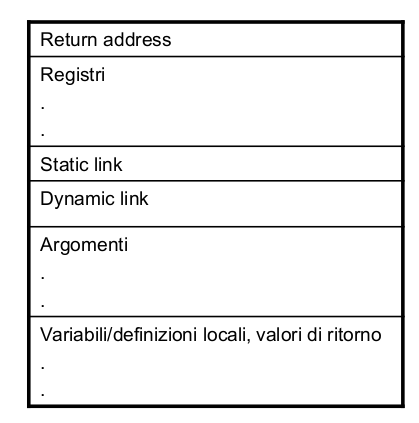
\includegraphics[scale=0.6]{img/act.png}
\end{center}
\newpage
Partiamo ora dal seguente codice in \textit{C}, e analizziamo i passaggi che avvengono nello stack:
\begin{minted}{C}
/* prima procedura */
int doppio(x) { 
	return 2 * x; 
}

/* seconda procedura, che chiama la prima */
int doppio_42(z) { 
	return doppio(z) - 42; 
}

/* chiamata nel main */
int r = doppio_42(42)
\end{minted} 
vediamo cosa accade nello stack:
si definiscono in ordine \textit{global frame e doppio\_42}, con i collegamenti di static link e dynamic link:
\begin{center}
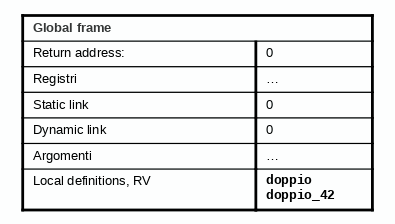
\includegraphics[scale=0.4]{img/sta1.png}
\quad 
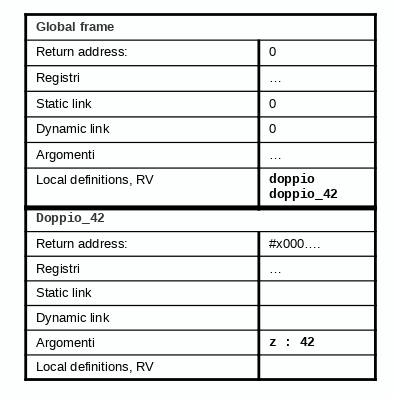
\includegraphics[scale=0.4]{img/sta2.png}
\quad
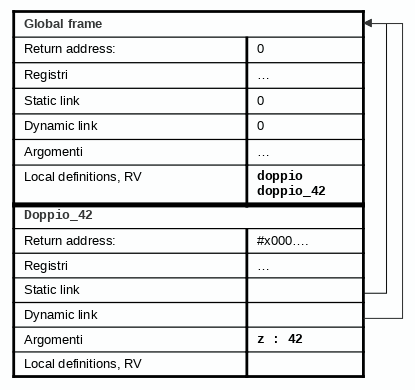
\includegraphics[scale=0.4]{img/sta3.png}
\end{center}
\newpage
Si aggiunge poi \textit{doppio}, con i collegamenti di static link e dynamic link:
\begin{center}
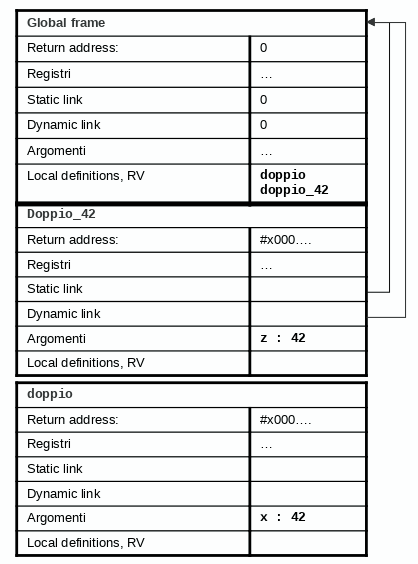
\includegraphics[scale=0.4]{img/sta4.png}
\quad 
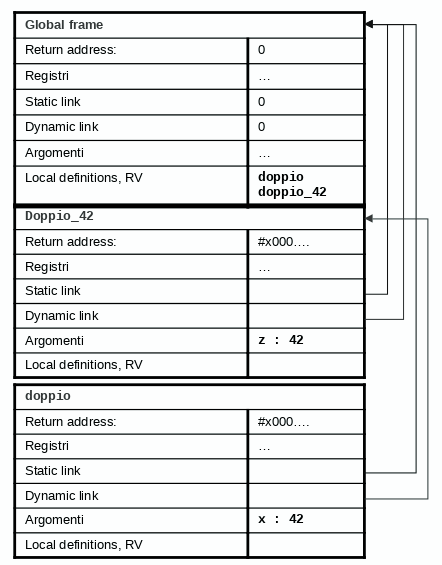
\includegraphics[scale=0.4]{img/sta5.png}
\end{center}
infine vengono risolti a partire da \textit{doppio}, salvando ogni volta i vari risultati nelle \textit{local definitions}:
\begin{center}
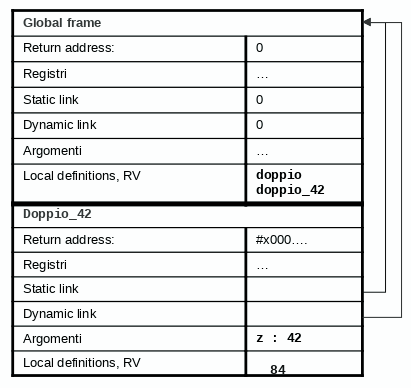
\includegraphics[scale=0.4]{img/sta6.png}
\quad
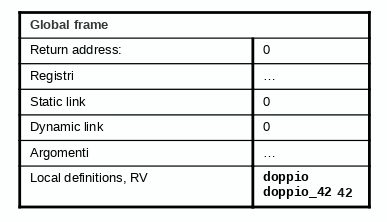
\includegraphics[scale=0.4]{img/sta7.png}
\end{center}
L'area di memoria per la manipolazione di strutture dati dinamiche verrà spiegata meglio al momento dell'introduzione delle primitive per la costruzione delle liste in Prolog e Lisp.\\
Il componente software che si occupa della gestione automatica della memoria in \textit{Lisp, Prolog, Java, C\#}, ed altri linguaggi è il \textit{garbage collector} (il servizio di raccolta rifiuti). \textit{C} e \textit{C++} non hanno un garbage collector standard.
\section{Logica}
Si ricordano le seguenti due definizioni:
\begin{enumerate}
\item \textbf{Implicazione}, indicata dal simbolo $\to$, è un connettivo logico che si usa per costruire forme logiche complesse. In una frase il \textit{se} comporta un'implicazione logica.
\item \textbf{Inferenza} è un meccanismo per il ragionamento. Detta anche \textit{modus ponens}, è una manipolazione sintattica (quindi non rappresentabile con tabelle di verità)
\end{enumerate}
Partiamo con l'esempio di una semplice dimostrazione geometrica effettuata con le regole della logica:
\begin{teorema}
Dato un triangolo isoscele (con $\overline{AB}=\overline{BC}$) si ha che $\angle A$, ovvero l'angolo in $A$, e $\angle C$, ovvero l'angolo in $C$, sono uguali.
\begin{center}
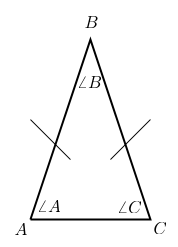
\includegraphics[scale=0.5]{img/tri.png}
\end{center}
\end{teorema}
\begin{proof}
Si comincia la dimostrazione con l'elenco delle conoscenze pregresse: 
\begin{enumerate}
\item se due triangoli sono uguali essi hanno lati e angoli uguali
\item se due triangoli hanno due lati e l'angolo sotteso uguale allora i due triangoli sono uguali
\item se viene definita la bisettrice di $\angle B$, $\overline{BH}$, si ha che $\angle ABH = \angle HBC$
\begin{center}
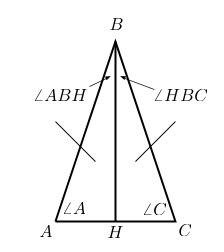
\includegraphics[scale=0.5]{img/tri2.png}
\end{center}
\end{enumerate}
Procediamo ora coi passi della dimostrazione:
\begin{enumerate}
\item $\overline{AB}=\overline{BC}$ per ipotesi
\item $\angle ABH = \angle HBC$ per la terza conoscenza pregressa
\item $\triangle HBC = \triangle ABH$ per la seconda conoscenza pregressa (dal secondo passo si ha che l'angolo tra la bisettrice, per forza uguale tra i due triangoli, e i due lati obliqui, uguali per ipotesi, è uguale per entrambi)
\item $\angle A= \angle C$ per la prima conoscenza pregressa (essendo uguali i triangoli per il passo precedente si ha che anche gli angoli sono uguali)
\end{enumerate}
Siamo così giunti alla fine della dimostrazione. Bisogna ora rappresentarla con gli strumenti della logica.\\
Sono stati svolti i seguenti passaggi:
\begin{itemize}
\item si è trasformata la seconda conoscenza pregressa in:\\\textbf{se} $\overline{AB}=\overline{BC}$ \textbf{e} $\overline{BH}=\overline{BH}$ \textbf{e} $\angle ABH = \angle HBC$ \textbf{allora} $\triangle ABH=\triangle HBC$
\item si è trasformata la prima conoscenza pregressa in:\\
\textbf{se} $\triangle ABH=\triangle HBC$ \textbf{allora} $\overline{AB}=\overline{BC}$ \textbf{e} $\overline{BH}=\overline{BH}$ \textbf{e} $\overline{AH}=\overline{HC}$ \textbf{e} $\angle ABH = \angle HBC$ \textbf{e} $\angle AHB = \angle CBH$ \textbf{e} $\angle A=\angle C$
\end{itemize}
Possiamo ora procedere col processo di \textbf{formalizzazione}, ovvero razionalizzare il processo per poter affermare:
$$\overline{AB}=\overline{BC}\,\vdash \angle A = \angle C$$
con $\vdash$ che è il simbolo di \textit{derivazione logica} e significa "consegue", "allora" etc...\\
Quindi per ottenere:
$$\overline{AB}=\overline{BC}\,\vdash \angle A = \angle C$$
abbiamo assunto:
$$P=\{\overline{AB}=\overline{BC},\,\angle ABH = \angle HBC,\,\overline{BH}=\overline{BH}\}$$
con queste conoscenze pregresse:
\begin{enumerate}
\item $\overline{AB}=\overline{BC}\wedge\overline{BH}=\overline{BH}\wedge\angle ABH = \angle HBC\to\triangle ABH=\triangle HBC$
\item  $\triangle ABH=\triangle HBC\to\overline{AB}=\overline{BC}\wedge\overline{BH}=\overline{BH}\wedge\overline{AH}=\overline{HC}\wedge\angle ABH = \angle HBC\wedge\angle AHB = \angle CBH\wedge\angle A=\angle C$
\end{enumerate}
Si ha quindi una catena di formule (\textbf{P} sono le ipotesi iniziali):
\begin{enumerate}
\item \textbf{P1:} $\overline{AB}=\overline{BC}$ preso da \textbf{P}
\item \textbf{P2:} $\angle ABH = \angle HBC$ preso da \textbf{P}
\item \textbf{P3:} $\overline{BH}=\overline{BH}$ preso da \textbf{P}
\item \textbf{P4:} $\overline{AB}=\overline{BC}\wedge\overline{BH}=\overline{BH}\wedge\angle ABH = \angle HBC$ preso da \textbf{P1, P2, P3} e dalla regola di inferenza detta \textbf{introduzione della congiunzione}
\item \textbf{P5:} $\triangle ABH=\triangle HBC$ da \textbf{P4}, dalla \textbf{regola 2} (\textit{se due triangoli hanno due lati e l'angolo sotteso uguale allora i due triangoli sono uguali}) e dalla regola di inferenza detta \textbf{modus ponens}
\item \textbf{P6:} $\overline{AB}=\overline{BC}\wedge\overline{BH}=\overline{BH}\wedge\overline{AH}=\overline{HC}\wedge\angle ABH = \angle HBC\wedge\angle AHB = \angle CBH\wedge\angle A=\angle C$ da \textbf{P5}, dalla \textbf{regola 1} (\textit{se due triangoli sono uguali essi hanno lati e angoli uguali}) e dalla regola di inferenza detta \textbf{modus ponens}
\item \textbf{P7:} $\angle A=\angle C$ da \textbf{P6} e dalla regola d'inferenza detta \textit{eliminazione della congiunzione} (date più asserzioni collegate da $\wedge$ posso eliderne un numero a piacere)
\end{enumerate}
Abbiamo così dimostrato tutto anche per mezzo dei costrutti della logica
\end{proof}
\begin{definizione}
Una dimostrazione del tipo \textit{F è conseguenza di S}, \textbf{dim}, si indica con:
$$S\,\,\vdash\,\, F$$
ed è una sequenza:
$$dim=<P_1,P_2,...,P_n>$$
con:
\begin{itemize}
\item $P_n=F$
\item $P_i\in S$ o con $P_i$ ottenibile dalle $P_1,...,P_{i-1}$ applicando una regola di inferenza
\end{itemize}
\end{definizione}
Un insieme di regole di inferenza costituisce la base di un calcolo logico e diversi insiemi di regole danno vita a diversi calcoli logici. Un calcolo logico ha lo scopo di manipolare le formule in modo unicamente sintattico, stabilendo una connessione tra un'insieme di formule di partenza, dette \textit{assiomi}, e un insieme di conclusioni.
\subsection{Logica Proporzionale}
La logica proposizionale si occupa delle conclusioni che si possono trarre da un insieme di proposizioni, che definiscono \textit{sintatticamente} la logica proposizionale (l'ultima parte della dimostrazione sopra è fatta da costrutti della logica proposizionale).\\
All'insieme \textbf{P} è associata una funzione di \textit{verità}, o di \textit{valutazione}, \textbf{V} (spesso indicata con \textbf{T} o \textbf{I}):
$$V:P\to\{vero,\,\,falso\}$$
che associa un valore di verità ad ogni eleemnto di \textbf{P}. La funzione di valutazione è il ponte di connessione tra sintassi e semantica in un linguaggio logico.\\
Le proposizione si combinano con i seguenti connettivi:
\begin{itemize}
\item \textbf{congiunzione:} $\wedge$
\item \textbf{disgiunzione:} $\vee$
\item \textbf{negazione:} $\neg$
\item \textbf{implicazione:} $\to$
\end{itemize}
L'insieme di tutte le formule formate dagli elementi di \textbf{P} e dalle loro combinazioni è detto: \textbf{Formule Ben Formate (FBF)}.\\
Le formule atomiche e i loro negativi vengono detti \textbf{letterali}. Il valore di verità di proposizione dipende dalla funzione di verità \textbf{V} e questa definizione può essere estesa sul dominio \textbf{FBF}:
\begin{itemize}
\item $V(\neg s)=non\,V(s)$
\item $V(a\wedge b)=V(a)\,\ e\,\, V(b)$
\item $V(a\vee b)=V(a)\,\ o\,\, V(b)$
\item $V(a\to b)=(non\,V(a))\,\ o\,\, V(b)$
\end{itemize}
ovvero, secondo la tavola di verità (con $1=vero$ e $0=falso$):
\begin{center}
\begin{tabular}{|c|c|c|c|c|c|c|}
\hline
$a$ & $b$ & $\neg a$ & $\neg b$ & $a\wedge b$ & $a\vee b$ & $a\to b$\\
\hline
1 & 1 & 0 & 0 & 1 & 1 & 1\\
\hline
1 & 0 & 0 & 1 & 0 & 1 & 1\\
\hline
0 & 1 & 1 & 0 & 0 & 1 & 0\\
\hline
0 & 0 & 1 & 1 & 0 & 0 & 1\\
\hline
\end{tabular}
\end{center}
La tavola di verità costituisce la semantica di un insieme di proposizioni mentre un calcolo logico dice come generare nuove formule logiche, ovvero espressioni sintattiche, a partire dagli assiomi. Questo calcolo deve garantire che le nuove formule generate siano vere se gli assiomi sono veri. Questo processo di generazione si chiama \textbf{dimostrazione}.\\
Per ottenere nuove formule dagli assiomi si usa il calcolo proposizionale, che si base su regole di inferenza. Una regola di inferenza ha la seguente forma:
$$\frac{F_1,F_2,...,F_N}{R}\,\,[\mbox{nome regola}]$$
con $F_i$ formula vera in \textbf{FBF} e $R$ è la formula vera generata da inserire in \textbf{FBF}. Vediamo qualche esempio:
\begin{esempio}[Modus Ponens]
$$\frac{a\to b,\,\,a}{b}$$
ovvero:
\begin{itemize}
\item Se piove, la strada è bagnata
\item Piove
\item Allora la strada è bagnata
\end{itemize}
Ovvero, la regola sintattica del modus ponens ci permette di
aggiungere le conclusioni di una “regola” al nostro insieme di formule ben formate “vere”
\end{esempio}
\begin{esempio}[Modus Tollens]
$$\frac{a\to b, \neg b}{\neg a}$$
ovvero:
\begin{itemize}
\item Se piove, la strada è bagnata
\item La strada non è bagnata
\item Allora non piove
\end{itemize}
Ovvero, la regola sintattica del modus tollens ci permette di
aggiungere la premessa negata di una “regola” al nostro insieme di formule ben formate “vere”
\end{esempio}
\begin{esempio}[Eliminazione e Introduzione di $\wedge$]
$$\frac{P_1\wedge P_2 \wedge ... \wedge P_n}{P_i}\,\,[\mbox{Eliminazione di }\wedge]$$
ovvero:
\begin{itemize}
\item Piove e la strada è bagnata
\item Piove
\end{itemize}
$$\frac{P_1, P_2,...,P_n}{P_1\wedge P_2 \wedge ... \wedge P_n}\,\,[\mbox{Introduzione di }\wedge]$$
ovvero:
\begin{itemize}
\item Piove
\item La strada è bagnata
\item Piove e la strada è bagnata
\end{itemize}
Ovvero, la regola sintattica dell’eliminazione della congiunzione ci permette di aggiungere all’insieme \textbf{FBF} i singoli componenti di una formula complessa. \\
Queste regole si chiamano anche, rispettivamente, \textit{di congiunzione} e \textit{di disgiunzione}
\end{esempio}
\begin{esempio}[Introduzione di $\vee$]
$$\frac{a}{a\vee b}$$
ovvero:
\begin{itemize}
\item Piove
\item Piove o c'è vita su Marte
\end{itemize}
Ovvero, la regola sintattica dell’introduzione della disgiunzione ci permette di aggiungere i singoli componenti di una formula.\\
Questa regola è detta anche \textit{di addizione}
complessa
\end{esempio}
\begin{esempio}
Ecco altre regole utili:
\begin{itemize}
\item \textbf{Terzo Escluso:}
$$\frac{a\vee\neg a}{vero}$$
\item \textbf{Eliminazione di} $\neg$:
$$\frac{\neg\neg a}{a}$$
\item \textbf{Eliminazione di} $\vee$:
$$\frac{a\vee vero}{a}$$
\item \textbf{Contraddizione:}
$$\frac{a\wedge\neg a}{b}$$
ovvero da una contraddizione posso trarre qualsiasi conseguenza
\end{itemize}
\end{esempio}
Queste regole di inferenza fanno parte del \textit{calcolo naturale}, detto anche \textit{di Gentzen}, ovvero il loro formalizzatore. Questo tipo di calcolo consiste nel formalizzare i modi di derivare conclusioni a partire dalle premesse, ovvero di derivare direttamente un FBF mediante una sequenza di passi ben codificati. La regola del \textit{modus ponens} (ovvero l'eliminazione dell'implicazione), insieme al principio del terzo escluso, posso essere usati anche \textit{procedendo per assurdo} alla dimostrazione di una data formula; questa procedura è detta \textit{principio di risoluzione}. Il \textit{principio di risoluzione} è una regola di inferenza generalizzata semplice e facile da utilizzare e implementare. Questo principio lavora su FBF trasformate in \textit{forma normale congiunta}, dove ogni congiunto è detto \textit{clausola}. L'osservazione alla base del principio è un'estensione della rimozione dell'implicazione sulla base del principio di contraddizione e si usa per dimostrazioni per assurdo:
$$\frac{p\vee r,\, s\vee r}{p\vee s}\,\,\,\,\,\,\,\,\,\,\frac{\neg r,\, r}{\perp}$$
dove:
\begin{itemize}
\item $p\vee s$ è la \textit{clausola risolvente}
\item $\perp$ è la \textit{clausola vuota}, che corrisponde all'aver creato una contraddizione con delle FBF (posso infatti dedurre qualsiasi cosa, anche la clausola vuota)
\end{itemize}
\newpage
vediamo un'altra regola di inferenza:
\begin{esempio}[(unit) resolution]
$$\frac{\neg p,\,\, q_1\vee q_2\vee ... \vee q_k \vee p}{q_1\vee q_2\vee ... \vee q_k}$$
o anche:
$$\frac{p,\,\, q_1\vee q_2\vee ... \vee q_k \vee \neg p}{q_1\vee q_2\vee ... \vee q_k}$$
è una regola di risoluzione molto generale e se una delle due clausole da risolvere è un \textit{letterale} (come negli esempi) si parla di \textit{unit resolution}. Come esempio di può avere:
\begin{itemize}
\item non piove, piove e c'è il sole
\item c'è il sole
\end{itemize}
\end{esempio}
Vediamo ora come funzionano le dimostrazioni per assurdo.\\
Si supponga di avere un'insieme di FBF vere e di avere una proposizione \textit{p} da dimostrare vera. Si ha il metodo \textit{reductio ad absurdum}:
\begin{itemize}
\item assumo $\neg p$ vera
\item se combinandola con le FBF ottengo una contraddizione allora $p$ deve essere vera (o meglio derivabile)
\end{itemize}
\begin{esempio}[provo che q è vera]
assumo:
\begin{itemize}
\item $FBF=\{p\to q,\,\,p,\,\,\neg w,\,\,e,\,\,r\}$
\item assumo vera $\neg q$
\end{itemize}
si ha che $FBF\cup \{\neg q\}$ genera una contraddizione infatti:
\begin{itemize}
\item $p\to q \equiv\neg p\vee q$ combinato con $p$ produce $q$ e quindi si ha $q\vee\neg q$, ovvero una contraddizione
\item se applico a $q$ e $\neg q$ il principio di risoluzione ottengo la clausola vuota $\perp$
\end{itemize}
\end{esempio}
Torniamo ad analizzare gli assiomi. Si hanno delle proposizioni sempre vere:
\begin{itemize}
\item $a\to(b\to a)$
\item $(a\to(b\to c))\to((a\to b)\to(a\to c))$
\item $(\neg b\to \neg a)\to ((\neg b\to a)\to b)$
\item $\neg(a\wedge \neg a)$ detto \textit{principio di non contraddizione}
\item $a\vee \neg a$ detto \textit{principio} del terzo escluso
\end{itemize}
Vediamo un esempio:
\begin{esempio}
Si ha la seguente affermazione:\\
\textit{se l'unicorno è mitico, allora è immortale, ma se non è mitico allora è mortale. Se è mortale o immortale, allora è cornuto. L'unicorno è magico se è cornuto.} Ho le seguenti domande:
\begin{enumerate}
\item l'unicorno è mitico?
\item l'unicorno è magico?
\item l'unicorno è cornuto?
\end{enumerate}
Bisogna quindi esprimere il problema con la logica delle proposizioni, individuare teoremi da dimostrare e infine dimostrarli. Le proposizioni saranno quindi:
\begin{itemize}
\item UM = unicordo è mitico
\item UI = unicorno è immortale
\item UMag = unicorno è magico
\item UC = unicorno è cornuto
\end{itemize}
che trascritto in logica diventa, che sono le mie conoscenze pregresse:
$$UM\to UI$$
$$\neg UM \to \neg UI$$
$$\neg UI\vee UI\to UC$$
$$UC\to Umag$$
dimostro ora le domande rappresentandole in forma logica. Si ha:
$$S=\{UM\to UI,\,\,\neg UM \to \neg UI,\,\,\neg UI\vee UI\to UC,\,\,UC\to Umag\}$$
con le domande che diventano:
\begin{itemize}
\item $S\vdash UM$?
\item $S\vdash Umag$?
\item $S\vdash UC$?
\end{itemize}
\newpage
Inizio a dimostrare la terza:\\
$$P1: \neg UI\vee UI\to UC\,\, \mbox{ da }S$$
$$P2: \neg UI\vee UI \mbox{ da }A5 \mbox{(tautologia)}$$
$$P3: UC\mbox{ da}P2,\,P2\,\, e\,\, ModusPonens$$
$P3$ si può scrivere già perché $P2$ è una tautologia, quindi posso utilizzare il modus ponens.\\
Ecco la seconda:\\
$$P4: UC\to Umag \mbox{ da }S$$
$$P5: Umag \mbox{ da }P3,\,P4\,\, e\,\, ModusPonens$$
Ed ecco la prima:\\
non è dimostrabile con queste conoscenze pregresse, non posso usare nessuna regola di inferenza
\end{esempio}
Si hanno differenze tra \textit{sintassi} e \textit{semantica}. L'operazione di derivazione $\vdash$ è un operatore sintattico e il calcolo logico fornisce una manipolazione sintattica e simbolica.\\ 
La semantica dipende dalla funzione di interpretazione, o funzione di valutazione o funzione di verità, $V$, che si basa sulle tabelle di verità. Si ha l'operatore di \textit{conseguenza logica} $\models$. Si ha, data una particolare logica che:
$$S\vdash f \mbox{ se e solo se } S\models f$$
Con $S$ insieme di formule iniziale e $f$ una FBF, il tutto in dipendenza da una funzione di verità $V$.\\
Una FBF vera indipendentemente dai valori dei letterali è detta \textit{tautologia}. Una particolare interpretazione $V$ che rende vere tutte le formule di $S$ è detta \textit{modello} di $S$.
\newpage
\subsection{Logica del primo ordine}
Di cui fanno parte i sillogismi (tutti gli uomini sono mortali, Socrate è mortale quindi Socrate è mortale). Si ha la \textit{logica proposizionale}, computazionalmente e semanticamente più chiara, ma limitata nella difficoltà di rappresentare asserzioni circa insiemi di elementi in maniera concisa. Nel sillogismo sopra la prima frase non è esprimibile in logica proposizionale. Si hanno le seguenti nozioni nella logica del primo ordine (LPO):
\begin{itemize}
\item variabile
\item costante
\item relazione (o predicato), che è un sottoinsieme di un prodotto cartesiano
\item funzione
\item quantificatore
\end{itemize}
quindi un linguaggio del primo ordine è costituito da \textit{termini} costruiti a partire da:
\begin{itemize}
\item \textit{V} insieme di simboli di variabili
\item \textit{C} insieme di simboli di costante
\item \textit{R} insieme di simboli di relazione o predicati di varia arità
\item \textit{F} insieme fi funzioni di varia arità
\item connettivi logici e simboli di quantificazione universale, $\forall$ (universale, "per ogni") e $\exists$(esistenziale, "esiste")
\end{itemize}
La costruzione di un linguaggio di primo ordine è \textit{ricorsiva}. I termini più semplici sono predicati
$$r\subseteq C_0\times C_1\times\cdots\times C_n$$
ovvero le relazioni cartesiane su \textit{C}, scritte come $r(c_1,...,c_n)$.\\
Le funzioni sono definite con dominio e codominio:
$$f:C_0\times C_1\times\cdots\times C_n\to C$$
e una funzione si scrive come $f(c_1,...,c_n)$.\\
Si hanno FBF costruite ricorsivamente da:
\begin{itemize}
\item un \textit{termine}, ovvero un elemento di \textit{C}, \textit{V} o l'applicazione di una funzione $f(t_1,t_2,...t_n)$
\item un termine costruito da un predicato $r(t_1,t_2,...t_n)$, con $t_i$ termini, appartiene ad una FBF
\item diversi elementi di FBF connessi da connettivi logici standard($\vee,\,\wedge,\,\neg,\,\to$) appartengono a FBF, tali combinazioni sono dette $t(t_1,t_2,...t_n)$
\item le formule $\forall x,\,t(t_1,t_2,...t_n)$ e $\exists x,\,t(t_1,t_2,...t_n)$ appartengono a FBF
\end{itemize}
Rivediamo ora il sillogismo \textit{tutti gli uomini sono mortali, Socrate è mortale quindi Socrate è mortale}. Ho:
\begin{itemize}
\item l'insieme delle costanti individuali $C=\{Sorate,\, Platone,\,...\}$
\item l'insieme dei predicati $P=\{uomo,\,mortale\}$
\end{itemize}
traduco quindi le asserzioni principali del sillogismo:
$$\forall x, (uomo(x)\to mortale(x))$$
$$uomo(Socrate)$$
e traduco la conclusione:
$$mortale(socrate)$$
Bisogna giustificare la semantica con nuove regole.\\
Si aggiunge una nuova regola d'inferenza per la logica dei predicati, l'eliminazione del quantificatore universale $\forall$ (\textit{C} insieme delle costanti):
$$\frac{\forall x, T(...,x,...), c\in C}{T(...,c,...)}$$
Quindi risolvo il sillogismo con questa regola:
$$\frac{(\forall x, uomo(x)\to mortale(x)), Socrate\in C}{uomo(Socrate)\to mortale(Socrate)}$$
poi applico il modus ponens, detto, per la logica proposizionale, anche \textit{eliminazione dell'implica} $\to$:
$$\frac{uomo(Socrate), uomo(Socrate)\to mortale(Socrate)}{mortale(Socrate)}$$
Abbiamo altre regole di inferenza per il quantificatore esistenziale:
\begin{itemize}
\item Introduzione del quantificatore esistenziale $\exists$:
$$\frac{T(...,c,...), c\in C}{\exists x, T(...,x,...)}$$
\item si hanno le seguente identità:
$$\exists x, \neg T(...,x,...)\equiv \neg\forall x, T)...,x,...)$$
$$\forall x, \neg T(...,x,...)\equiv \neg\exists x, T(...,x,...)$$
\end{itemize}
\chapter{Prolog}
Il prolog è un linguaggio logico rappresentato da una semplicità del formalismo, è di alto livello e ha una semantica chiara. Un programma è un insieme di formule e si ha come fine la dimostrazione di un'affermazione. La base formale è data dalle \textit{clausole di Horn} e dal meccanismo di \textit{risoluzione}. Prolog viene da \textit{PROgramming LOGic} e si basa su una restrizione della logica del primo ordine e usa uno stile dichiarativo. Si vuole determinare la veridicità di una affermazione. Ogni FBF può essere in \textit{forma normale a clausola}:
\begin{itemize}
\item \textit{formula normale congiunta:} congiunzione di disgiunzioni o di negazione di predicati (sia positivi che negativi):
$$\wedge_i(\vee_iL_{ij})$$
\begin{esempio}
ecco degli esempi:
\begin{itemize}
\item $(p(x)\vee q(x,y)\vee \neg t(z))\wedge(p(w)\vee\neg s((u)\vee \neg r(v))$
\item $(\neg t(z))\vee (p(w)\vee\neg s(u))\wedge (p(x)\vee s(x)\vee q(y))$
\end{itemize}
che sono riscrivibili come:
$$t(z)\to p(x)\vee q(x,y)$$
e
$$s(u)\wedge r(v)\to p(w)$$
\end{esempio}
\item \textit{forma normale disgiunta}: disgiunzione di congiunzioni o di negazione di predicati (sia positivi che negativi)
$$\vee_i(\wedge_iL_{ij})$$
\end{itemize}
Le clausole con un solo letterale positivo solo le \textit{clausole di Horn} e un programma in prolog è una collezione di \textit{clausole di Horn}. Non tutte le FBF possono essere \textit{clausole di Horn}.\\
Prolog non ha istruzioni. Si hanno \textit{fatti} (asserzioni vere nel contesto descritto) e \textit{regole}.\\
%aggiungi roba
Parliamo di sintassi:
\begin{itemize}
\item ":-" è l'implicazione
\item tutto termina con un punto "."
\item la "," è l'and logico
\item il ";" è lor logico
\item \textit{a.} è un fatto o asserzione
\item \textit{b :- c, d, ... .} è una regola (c, d, ... termini composti)
\item \textit{? :- x, y, ... .} è un goal o una query (x, y, ... termini composti)
\item non si dichiarano variabili e si ha solo la lista come struttura dati. SI hanno vari termini (atomi variabili etc...):
\begin{itemize}
\item atomi (numeri, ...) ovvero caratteri alfanumerici che inizia col carattere minuscolo (puo esserci \_ ma quindi non un numero), qualsiasi cosa dentro apici "" o numeri.
\item variabili è un carattere che inizia con la maiuscola (e quindi non con un numero) o col carattere \_ (che indica una variabile anonima o \textit{indifferenza}). Le variabili si istanziano (non con un assegnamento) col procedere del programma e della dimostrazione
\item termine composto (col simbolo +). Un \textit{funtore} è un simbolo di funzione o predicato che applica ad argomenti, messi tra parentesi tonde (da non spaziare dal funtore). Il funtore è minuscolo e non è un numero
\end{itemize}
\item un \textit{fatto} è un nome di predicato che inizia con la maiuscola
\item una \textit{regola} esprime la dipendenza di un fatto da un insieme di altri fatti. Possono esprimere anche definizioni
\item una regola ha una \textit{testa (head)}, ed è il conseguente e un \textit{corpo (body)}, l'antecedente. Si ha quindi un solo termine come conseguente (\textit{regola di Horn}). Si ha quindi:
\textit{un pesce è un animale e ha le squame}: 
\begin{minted}{prolog}
pesce(x) :- animale(x), ha_le_squame(x).
\end{minted}
%oppure:\\
%\textit{gigi ama chiunque ami il vino}
%aggiungi prolog
\item una relazione si può esprimere con più regole:
\begin{minted}{prolog}
genitore(x, y) :- padre(x,y).
genitore(x, y) :- madre(x,y).
\end{minted}
\item si ha la ricorsione per definire una relazione. La definizione richiede almeno due proposizioni, \textit{caso base} e \textit{caso generale}:
\begin{minted}{prolog}
antenato(x, y) :- genitore(x, y).
antenato(x, y) :- genitore(z, y), antenato(x, z).
\end{minted}
\item i commenti in linea si hanno con \% e su più linee con /* e */
\begin{minted}{prolog}
%commento
antenato(x, y) :- genitore(x, y).
antenato(x, y) :- genitore(z, y), antenato(x, z).
/*commento
su più righe*/
\end{minted}
\item il prompt ci chiede una FBF di Horn con "?-" (senza variabili) e prende l'input e come output si avrà \textit{yes}. Interrogare il programma è richiedere una dimostrazione. Se si chiede una formula presente direttamente si avrà subito \textit{yes} (se il goal è una clausola (un fatto) quindi si applica il principio di risoluzione e si ha la dimostrazione effettuata). In un'interrogazione si possono avere \textit{variabili esistenziali}. Tutte le variabili istanziate sono mostrate in risposta
\item l'operatore di istanziazione di variabili durante la prova di un predicato è il risultato di una procedura particolare, detta \textit{unificazione}
\item dati due termini la procedura di unificazione crea un insieme di sostituzioni delle variabili. Questo insieme permette di rendere uguali i due termini. Tradizionalmente si ha il \textit{most general unifier (Mgu)}. Una sostituzione è indicata come una sequenza ordinata di coppie \textit{variabile/valore}:
\begin{minted}{prolog}
Mgu(42, 42) % ->{} non serve nessuna sostituzione
Mgu(42, X) % ->{X/42} ovvero X deve essere 42
Mgu(X,42) % ->{X/42} ovvero X deve essere 42
Mgu(foo(bar, 42), foo(bar, X)) % ->{X/42} ovvero X deve essere 42
Mgu(foo(X, 42), foo(bar, X)) % ->{Y/bar, X/42} ovvero X deve essere 42

Mgu(foo(bar(42), baz), foo(X, Y))  /* ->{X/bar (42), Y/baz}
 ovvero X deve essere  bar(42) e Y baz*/
Mgu(foo(X), foo(bar(Y))) 
Mgu(foo(bar(42), baz), foo(X, Y))  /* ->{X/bar (y), Y_:G001}
 ovvero non si ha soluzione */
\end{minted}
L'Mgu non è altro che il risultato finale della procedura di valutazione del Prolog. Il modo più semplice per vedere se l'unificazione funziona è usare "=", ovvero, ricollegandoci al codice sopra:
\begin{minted}{prolog}
?- 42 = 42.
Yes

?- 42 = X.
X = 42 % per rendere vera l'affermazione serve x = 42
Yes

?- foo(bar, 42) = foo(bar, X).
X = 42
Yes

?- foo(Y, 42) = foo(bar, X).
Y = bar
X = 42
Yes

?- foo(bar(42), baz) = foo(X, Y).
X = bar(42)
Y = baz
Yes

?- foo(X) = foo(bar(Y)).
X = bar(Y)
Y = _G001
Yes

?- foo(42, bar(X), trillian) = foo(Y, bar(Y), X).
No
\end{minted}
\begin{esempio}
\textit{Si descrive un insieme di fatti riguardanti i corsi offerti:}\\
Tutte le informazioni sono concentrate in una relazione a 6 campi:
\begin{minted}{prolog}
corso(linguaggi, lunedì, ’9:30’, ’U4’, 3, antoniotti).
corso(biologia_computazionale, lunedì, ’14:30’, ’U14’, t023, antoniotti).
\end{minted}
a partire da qui costruisco altri predicati:
\begin{minted}{prolog}
aula(Corso, Edificio, Aula) :-
	corso(Corso, _, _, Edificio, Aula, _).
docente(Corso, Docente) :-
	corso(Corso, _, _, _, _, Docente).
\end{minted}
oppure posso concentrare le informazioni in una relazione con 4 campi; le informazioni sono concentrate in termini funzionali che rappresentano le informazioni raggruppate logicamente;
\begin{minted}{prolog}
corso(linguaggi, orario(lunedì, ’9:30’), aula(’U4’, 3), antoniotti).
corso(biologia_computazionale,
	orario(lunedì, ’14:30’),
	aula(’U4’, 3),
	antoniotti).
\end{minted}
posso quindi definire altri predicati:
\begin{minted}{prolog}
aula(Corso, Edificio, Aula) :- corso(Corso, _, aula(Edificio, Aula), _).
docente(Corso, Docente) :- corso(Corso, _, _, Docente).

% oppure...

aula(Corso, Luogo) :- corso(Corso, _, Luogo, _).
\end{minted}
oppure ancora i predicati che abbiamo definito a partire dalle relazioni con 6 o 4 campi possono essere ricodificate con predicati binari:
\begin{minted}{prolog}
giorno(linguaggi, martedì).
orario(linguaggi, ’9:30’).
edificio(linguaggi, ’U4’).
aula(linguaggi, 3).
docente(linguaggi, antoniotti).
\end{minted}
La relazioni a 6 o 4 argomenti possono essere ricostruite in a partire da queste relazioni binarie. La costruzione di schemi \textit{RDF/XML} (e, a volte,\textit{ SQL}) corrisponde a questa operazione di ri-rappresentazione
\end{esempio}
\item Si definisce una lista in Prolog racchiudendo gli elementi (termini e/o variabili logiche) della lista tra parentesi quadre \textit{[} e \textit{]} e separandoli da virgole. Gli elementi di una lista in Prolog possono essere termini
qualsiasi o liste. La lista vuota si indica con \textit{[]}. Una coda non vuota si può dividere in \textit{testa} e \textit{coda}:
\begin{itemize}
\item la testa è il primo elemento della lista
\item la coda rappresenta tutto il resto ed è sempre una lista
\end{itemize}
\begin{minted}{prolog}
[a, b, c] % a è la testa e [b, c] la coda
[a, b] % a è la testa e [b] la coda
[a] % a è la testa e [] la coda
[[a]] % [a] è la testa e [] la coda
[[a, b], c] % [a, b] è la testa e [c] la coda
[[a, b], [c], d] % [a, b] è la testa e [[c], d] la coda
\end{minted}
Prolog possiede uno speciale operatore usato per distinguere tra l'inizio e la coda di una lista: l'operatore \textit{|}:
\begin{minted}{prolog}
?- [X | Ys] = [mia, vincent, jules, yolanda].
X = mia
Ys = [vincent, jules, yolanda]
Yes

?- [X, Y | Zs] = [the, answer, is, 42].
X = the
Y = answer
Zs = [is, 42]
Yes

?- [X, 42 | _] = [41, 42, 43, foo(bar)].
X = 41
Yes
\end{minted}
La lista vuota \textit{[]} in prolog è gestita come una lista speciale:
\begin{minted}{prolog}
?- [X | Ys] = [].
No
\end{minted}
\item La base di conoscenza è nascosta ed è accessibile solo tramite opportuni comandi o tramite ambiente di programmazione. Bisogna poter caricare un insieme di fatti e regole. Per farlo si ha il comando \textit{consult}, che appare come un predicato da valutare (un goal) e prende almeno un termine che denota un file come argomento, file che deve contenere fatti e regole
\begin{minted}{prolog}
?- consult(’guida-astrostoppista.pl’).
Yes

?- consult(’Projects/Lang/Prolog/Code/esempi-liste.pl’).
Yes
\end{minted}
\item il predicato \textit{consult} può essere usato anche per inserire fatti e regole direttamente alla console usando il termine speciale \textit{user}:
\begin{minted}{prolog}
?- reconsult(’guida-astrostoppista.pl’).
Yes
% A questo punto la base di dati Prolog contiene il
% nuovo contenuto del file.
\end{minted}
il predicato \textit{reconsult} deve invece essere usato quando si vuole ricaricare un file (ovvero un data o knowledge base) nell'ambiente Prolog. L’effetto è di prendere i predicati presenti nel file, rimuoverli completamente dal data base interno e di reinstallarli utilizzando le nuove definizioni:
\begin{minted}{prolog}
?- reconsult(user). % Notare il sotto-prompt.
|- foo(42).
|- friends(zaphod, trillian).
|- ^D
Yes

% A questo punto la base di dati Prolog contiene i due
% fatti inseriti manualmente.
?- friends(zaphod, W).
W = trillian
Yes
\end{minted}
\item Prolog lavora anche su strutture ad albero e anche i programmi sono strutture dati manipolabili con predicati \textit{extra-logici}. Si ha la ricorsione e non l'assegnamento. Un programma Prolog è un insieme di clausole di Horn che rappresentano:
\begin{itemize}
\item fatti riguardanti gli oggetti in esame e le relazioni che intercorrono tra di loro
\item regole sugli oggetti e sulle relazioni (se ... allora ...)
\item interrogazioni (goals o queries; clausole senza testa), sulla base della conoscenza definita
\end{itemize}
\item si ha l'implicazione: 
$$\neg B \vee A \mbox{ corrisponde a } B\to A$$
data una clausola $A\vee ... \vee A_n\vee \neg B_1\vee ... \vee\neg B_n$, usando De Morgan si ottiene:
$$(A\vee ... \vee A_n)\vee \neg (B_1\vee ... \vee B_n)$$
$$\downarrow$$
$$(B\vee ... \vee B_n)\to (A_1\vee ... \vee A_n)$$
\textit{si può fare anche l'inverso}.\\
\end{itemize}
vediamo un programma che fa la somma tra due naturali:
\begin{minted}{prolog}
sum(0, X, X).
sum(s(X), y, s(Z)) -: sum(X, Y, Z).
\end{minted}
con $S(n)$ interpretato come il successore ($0=0,\, s(0)=1, \,s(s(0))=2,... $).\\
Quando viene specificato un goal esso viene confrontato con tutte le clausole di programma, che usa il procedimento di negazione e di trasformazione in sintassi Prolog.\\
Vediamo i passi:
\begin{itemize}
\item  interroghiamo il programma:
$$\exists X\,\,\, sum(s(0),\, 0,\, X)\,\,\,\,\,\{X\,/\, s(0)\}$$
$$\exists W\,\,\, sum(s(s(0)),\, s(0), \, W)\,\,\,\,\,\{W\,/\, s(s(s(0)))\}$$
dove $\{X\,/\, s(0)\}$ e $\{W\,/\, s(s(s(0)))\}$ sono le sostituzioni che rappresentano il risultato
\item usiamo il procedimento di negazione e trasformazione in sintassi:
\begin{minted}{prolog}
:- sum(s(0), 0, N).    %{N / s(0)}
:- sum (s(s(0)), s(0), W).     %{W / s(s(s(0)))}
\end{minted}
con $\{N\, /\, s(0)\}$ e $\{W \,/\, s(s(s(0)))\}$ che sono le \textbf{sostituzioni}. Una sostituzione ci dice che valori (che possono essere altre variabili) si può sostituire le variabili di un termine. Una sostituzione si indica con $\sigma=\{X_1\,/\,V_1/,..., X_k\,/\,V_k\}$ e può essere considerata come una funzione ($\sigma: T\to T$) applicabile ad un termine dell'insieme dei termini $T$.
\begin{esempio}
data la sostituzione $\sigma=\{X\,/\,42,\,Y\,/\, foo(s(0))\}$ si ha:
$$\sigma(bar(X,\,Y))=bar(42, \, foo(s(0)))$$
\end{esempio}
\end{itemize}
\newpage
\textit{Una computazione corrisponde al tentativo di dimostrare, tramite la regola di risoluzione, che una formula segue logicamente da un programma (è un teorema)}. Si ha inoltre che si deve determinare una sostituzione per le variabili del goal (le \textit{query}) per cui la query segue  logicamente dal programma:
\begin{esempio}
Sia dato il programma P e la query:
\begin{minted}{prolog}
:- p(t1, t2, ..., tm).
\end{minted}
se \textbf{X1,..., Xn} sono le variabili in \textbf{t1,..., tm}, il significato della query è:
$$\exists X1,\,..., \,Xn\, . \,p(t1, t2, ..., tm)$$
e si cerca una sostituzione:
$$s=\{X1\,/\,s1,...,\, Xn\,/\,sn$$
con gli $s\,i$ termini tali per cui:
$$P\vdash s[p(t1, t2, ..., tm)]$$
\end{esempio}
Dato un insieme di clausole di Horn è possibile derivare la clausola vuota solo se c'è almeno una clausola senza testa, ovvero se si ha una query $G_0$ da provare. Ovvero si deve dimostrare che da $P\cup G_0$ si può derivare la clausola vuota. Si dimostra per assurdo col principio di risoluzione.
\subsubsection{Risoluzione ad Input Lineare (SLD)}
Il sistema Prolog dimostra la veridicità di un goal eseguendo una sequenza di passi di risoluzione (l'ordine con cui vengono eseguiti questi passi rende i sistemi di prova basati sulla risoluzione più o meno efficienti). In Prolog la risoluzione avviene sempre fra l’ultimo goal derivato in ciascun passo e una \textit{clausola di programma} e mai fra due clausole di programma o fra una clausola di programma ed un goal derivato in precedenza. Questa forma di risoluzione è detta\textit{Risoluzione-SLD}  (\textit{Selection function for Linear and Definite sentences Resolution}), dove le sentenze lineari sono le clausole di Horn.
\begin{esempio}
partiamo dal goal $G_i$:
$$G_i\equiv \,\,\,?-\, A_{i,\, 1}, ...,  A_{i,\, m}.$$
e dalla regola:
$$A_r\,\,\,:-\,\,\, B_{r,\,1},..., B_{r,\,k}.$$
se esiste un unificatore $\sigma$ tale che $\sigma[A_r]=\sigma[A_{i,\,1}]$ allora si ottiene il nuovo goal:
$$G_{i+1}\equiv\,\,\,B^{'}_{r,\,1},..., B^{'}_{r,\,k},A^{'}_{i,\, 1}, ...,  A^{'}_{i,\, m}.$$
che è un passo di risoluzione eseguito dal sistema Prolog (con $\sigma[A_{i,\,m}]=A^{'}_{i,\,m}$ 4 $\sigma[B_{i,\,m}]=B^{'}_{i,\,m}$. \textit{La scelta di unificare il primo sottogoal di }$G_i$\textit{ è arbitraria (si sarebbe potuto scegliere, per esempio} $A_{i,\,m}$ \textit{o} $A_{i,\,c}$ \textit{con} $ c\in[1,\,m]$ \textit{)}
\end{esempio}
\begin{esempio}
partiamo dal goal $G_i$:
$$G_i\equiv \,\,\,?-\, A_{i,\, 1}, ...,  A_{i,\, m}.$$
e dalla regola (ovvero dal \textbf{fatto}):
$$A_r.$$
se esiste un unificatore $\sigma$ tale che $\sigma[A_r]=\sigma[A_{i,\,1}]$ allora si ottiene il nuovo goal:
$$G_{i+1}\equiv\,\,\,A^{'}_{i,\, 2}, ...,  A^{'}_{i,\, m}.$$
che ha dimensioni minori di $G_i$ avendo $m-1$ sottogoal
\end{esempio}
Nella risoluzione SLD, il passo di risoluzione avviene sempre fra l'ultimo goal e una clausola di programma. SI possono avere i seguenti risultati:
\begin{itemize}
\item \textbf{successo:} si genera la clausola vuota, ovvero se per $n$ finito $G_n$ è uguale alla clausola vuota $G_:n\equiv\,\,\,:-$
\item \textbf{insuccesso finito}: se per $n$ finito $G_n$  non è uguale alla clausola vuota $G_:n\equiv\,\,\,:-$ e non è più possibile derivare un nuovo \textit{risolvente} da $G_n$ ed una clausola d programma
\item \textbf{successo infinito: }se è sempre possibile derivare nuovi risolventi tutti diversi dalla clausola vuota
\end{itemize}
La \textbf{sostituzione di risposta} è la sequenza di unificatori usati; applicata alle variabili nei termini del goal iniziale dà la risposta finale.\\
Durante il processo di generazione di goal intermedi si costruiscono delle varianti dei letterali e delle clausole coinvolti mediante la\textit{ rinominazione di variabili}. Una variante per una clausola $C$ é la clausola $C^{'}$ ottenuta da $C$ rinominando le sue variabili, \textit{renaming}:
\begin{esempio}
\begin{minted}{prolog}
p(X) :- q(X, g(Z)).
% è uguale alla clausola con variabili rinominate:
p(X1) :- q(X1, g(FooFrobboz)).
\end{minted}
\end{esempio}
Possono esserci più clausole di programma utilizzabili per applicare la risoluzione con il goal corrente ed esistono diverse strategie di ricerca:
\begin{itemize}
\item \textbf{in profondità (Depth First)}: si sceglie una clausola e si mantiene fissa questa scelta, finché non si arriva alla clausola vuota o alla impossibilità di fare nuove risoluzioni; in questo ultimo caso si riconsiderano le scelte fatte precedentemente
\item \textbf{in ampiezza (Breadth First)}: si considerano in parallelo tutte le possibili alternative
\end{itemize}
\textbf{IL PROLOG ADOTTA UNA STRATEGIA DI RISOLUZIONE IN PROFONDITÀ CON \textit{BACKTRACKING}}.\\
Si ha così risparmio di memoria anche se non è una strategia completa per le clausole di Horn.\\
\subsubsection{Alberi di Derivazione}
Dato un programma logico $P$, un goal $G_i$ e una regola di calcolo $R$ si ha che un \textit{albero SLD} per $P\cup G_i$ via $R$ è definito sulla base del processo di prova visto precedentemente:
\begin{itemize}
\item ciascun \textbf{nodo} dell'albero è un goal (possibilmente vuoto)
\item la \textbf{radice }dell'albero SLD è il goal $G_0$
\item dato il nodo:
$$:-\,\,\, A_1,...,A_{m-1},A_m,A_{m+1},...,A_k$$
se $A_m$ è il sottogoal selezionato dalla regola di calcolo $R$, allora questo nodo (genitore) ha un nodo figlio per ciascuna clausola del tipo:
$$C_i\equiv A_i\,\,\, :-\,\,\, B_{i,\,1},...,B_{i,\,q}$$
$$C_k\equiv A_k$$
di $P$ tale che $A_i$ e $A_M$ ($A_K$ e $A_m$) sono unificabili attraverso la sostituzione più generale $\sigma$.\\
Il nodo figlio è etichettato con la clausola goal
$$:-\,\,\,\sigma[A_1,...,A_{m-1},B_{i,\,i},...,B_{i,\,q},A_{m+1},...,A_k]$$
$$:-\,\,\,\sigma[A_1,...,A_{m-1},A_m,A_{m+1},...,A_k]$$
e il ramo dal nodo padre al figlio è etichettato dalla sostituzione $\sigma$ e dalla clausola selezionata $C_i$ o $C_k$.\\
Il nuovo nodo $:-$ non ha figli.
\end{itemize}
La regola $R$ è variabile. Si ha:
\begin{itemize}
\item \textbf{regola Left-most}: ovvero si ha la scelta del sottogoal più a sinistra 
\item \textbf{regola Right-most}: ovvero si ha la scelta del sottogoal più a destra
\item si può avere la scelta di un sottogoal a caso
\item se si ha un modo per decider il miglior sottogoal  
\end{itemize}
\textbf{IL PROLOG ADOTTA UNA REGOLA LEFT-MOST}
\\
L'albero SLD (implicito!) generato dal sistema Prolog ordina i figli di un nodo secondo l'ordine dall'alto verso il basso delle regole e dei fatti del programma P. 
\begin{esempio}
Ecco un esempio:
\begin{center}
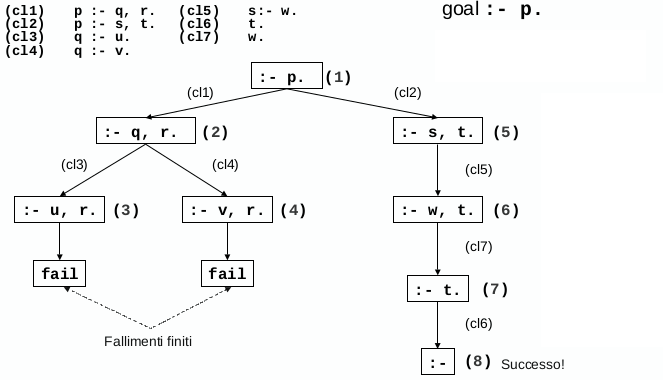
\includegraphics[scale=0.7]{img/alb.png}
\end{center}
\end{esempio}
Ad ogni ramo di un albero SLD corrisponde una derivazione
SLD e o gni ramo che termina con il nodo vuoto $:-$ rappresenta una derivazione SLD di successo. La regola di calcolo influisce sulla struttura dell'albero per quanto riguarda sia l'ampiezza sia la profondità tuttavia non influisce su correttezza e completezza; quindi, qualunque sia $R$, il numero di cammini di successo (se in numero finito) è lo stesso in tutti gli alberi SLD costruibili per $P\cup \{G_0\}$ e $R$ influenza solo il numero di cammini di fallimento (finiti ed infiniti).
\begin{esempio}
Ecco un altro esempio, con fallimento infinito, dove la clausola vuota può essere generata ma il Prolog non è in grado di trovare questa soluzione dato che la sua strategia di percorrimento dell’albero (implicito) di soluzioni è depth-first con backtracking :
\begin{center}
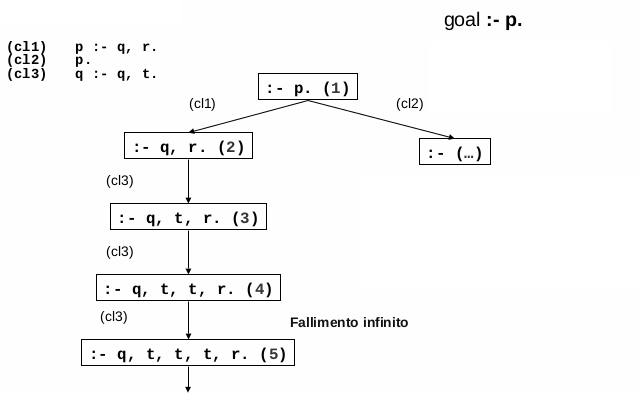
\includegraphics[scale=0.7]{img/alb2.png}
\end{center}
\end{esempio}
\end{document}